
\documentclass[border=10pt]{standalone}
\usepackage[table]{xcolor}
\usepackage{amsmath,amssymb,amsfonts,mathtools,bm}
\usepackage{booktabs,array}
\usepackage{tikz}
\usetikzlibrary{arrows.meta,positioning,calc,backgrounds,fit,shapes.geometric,decorations.pathreplacing}
\usepackage{pgfplots}
\pgfplotsset{compat=1.18}
\definecolor{sbnavy}{HTML}{1A2A4F}
\definecolor{sbteal}{HTML}{1C7293}
\definecolor{sbaccent}{HTML}{B5651D}
\definecolor{sbgrey}{HTML}{8A94A6}
\definecolor{sblight}{HTML}{EAF1F5}
\newcommand{\cmark}{\textcolor{sbteal}{\ensuremath{\boldsymbol{\checkmark}}}}
\newcommand{\xmark}{\textcolor{sbgrey}{\ensuremath{\boldsymbol{\times}}}}
\newcommand{\eqcol}{\color{sbnavy}}
\begin{document}
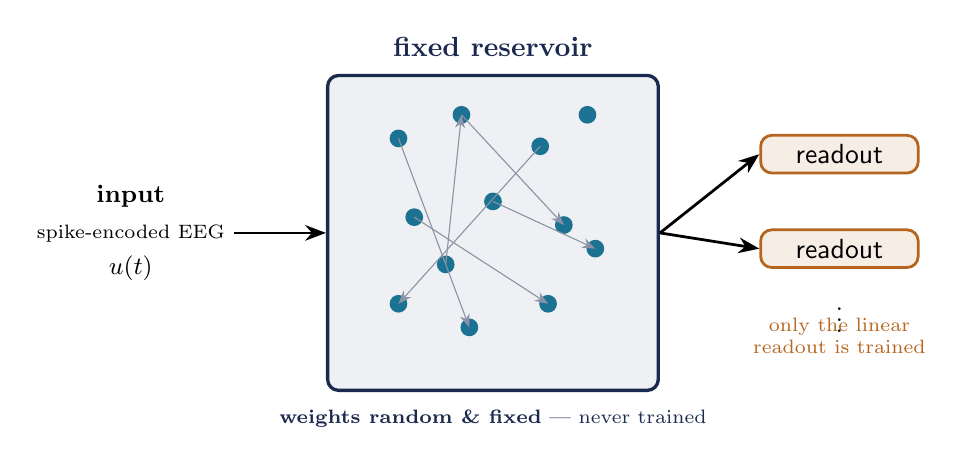
\begin{tikzpicture}[font=\sffamily,>=Stealth]
  \node[align=center,font=\small] (in) at (0,0) {\textbf{input}\\[2pt]{\scriptsize spike-encoded EEG}\\[2pt]$u(t)$};
  \node[draw=sbnavy,line width=1.2pt,rounded corners,fill=sbnavy!7,minimum width=4.2cm,minimum height=4.0cm] (res) at (4.6,0) {};
  \node[above=1mm of res,sbnavy,font=\bfseries] {fixed reservoir};
  \foreach \p in {(3.4,1.2),(4.2,1.5),(5.2,1.1),(5.8,1.5),(3.6,0.2),(4.6,0.4),(5.5,0.1),(3.4,-0.9),(4.3,-1.2),(5.3,-0.9),(5.9,-0.2),(4.0,-0.4)}{
     \fill[sbteal] \p circle (3.2pt);}
  \draw[sbgrey,->] (3.4,1.2)--(4.3,-1.2);
  \draw[sbgrey,->] (4.2,1.5)--(5.5,0.1);
  \draw[sbgrey,->] (4.6,0.4)--(5.9,-0.2);
  \draw[sbgrey,->] (3.6,0.2)--(5.3,-0.9);
  \draw[sbgrey,->] (4.0,-0.4)--(4.2,1.5);
  \draw[sbgrey,->] (5.2,1.1)--(3.4,-0.9);
  \node[below=1mm of res,align=center,font=\scriptsize,sbnavy] {\textbf{weights random \& fixed} --- never trained};
  \node[draw=sbaccent,line width=1pt,rounded corners,fill=sbaccent!12,minimum width=2cm] (r1) at (9.0,1.0) {readout};
  \node[draw=sbaccent,line width=1pt,rounded corners,fill=sbaccent!12,minimum width=2cm] (r2) at (9.0,-0.2) {readout};
  \node[font=\small] at (9.0,-1.0) {$\vdots$};
  \draw[->,line width=1pt] (in.east) -- (res.west);
  \draw[->,line width=1pt] (res.east) -- (r1.west);
  \draw[->,line width=1pt] (res.east) -- (r2.west);
  \node[below=5mm of r2,align=center,font=\scriptsize,sbaccent] {only the linear\\ readout is trained};
\end{tikzpicture}
\end{document}